\section{Grid graphs}
A comprehensive performance evaluation of the \textsf{SGL} algorithm was
conducted considering grid graph models with 64 nodes denoted as
$\mathcal{G}^{(64)}_{\mathsf{grid}}$.
We compare the performance of the \textsf{SGL} algorithm against state-of-the-art algorithms, namely
\textsf{CGL}, \textsf{CGL}$(\mathbf{A})$. We recollect that \textsf{CGL}$(\mathbf{A})$ stands for the
$\textsf{CGL}$ algorithm equipped with knowledge of the connectivity matrix $\mathbf{A}$, which gives
the exact information of which nodes are connected to which ones.

The experimental setup is as follows. The edges of the graph model are sampled from $\mathsf{Uniform}(0.1, 3)$.
The Laplacian matrix estimation is carried out on the basis of $T$ samples distributed according to
$\mathcal{N}(\mathbf{0}, \mathbf{L}_{\mathsf{grid}}^{\dagger})$. We repeat that experiment 20 times
for every value of $T$ and we average out the relative errors and F-scores\footnote{For the computation of the
F-score, we ignore edge weight values which are less than $10^{-1}$.}.

Some hyperparameter tunning is required. For the \textsf{SGL} algorithm, we fix
$\beta = 10$ for the values of $T$ such that $T / N > 5$. Otherwise, we start with
$\beta = 10^{-2}$, and we exponentially increase it up to $\beta = 4$.
Additionally, we fix $\alpha = 0$.

For the \textsf{CGL} and \textsf{CGL}$(\mathbf{A})$ algorithms, we follow the recipe by
Eglimez, i.e., we choose $\alpha$ from $\left\{0\right\}\cup\left\{0.75^{r}\left(s_{\text{max}}
\sqrt{\log(N) / T}\right) | r = 1, 2, ..., 14\right\}$, such that the relative error between
the estimated Laplacian and the ground truth is minimized, where $s_{\text{max}}$ is the
maximum value among the off-diagonal elements of the sample  covariance matrix.

Figure~\ref{fig:performance-grid} compares the performance of the algorithms for different
sample size regimes for the grid graph model. As it can be noted, the \textsf{SGL} algorithm outperforms the \textsf{CGL}
in both relative error and F-score senses. More precisely, for the case when the sample size is equal
to the number of nodes, the difference in relative error and in F score are around $12\%$ and $23\%$,
respectively.

As expected, with the additional prior knowledge of the connectivity matrix $\mathbf{A}$,
the \textsf{CGL}$(\mathbf{A})$ algorithm basically attains a perfect F-score for $T / N \geq 10$.
However, the connectivity matrix is not always available in practical problems, especially in clustering
tasks where the goal is precisely to understand the connectivity membership among the nodes.

Nonetheless, the proposed \textsf{SGL} algorithm presents a comparable performance against \textsf{CGL}$(\mathbf{A})$.
For instance, at $T/N = 5$, the difference in relative error is only around $2.5\%$, and it keeps decreasing
even further until virtually equal performance after $T / N = 100$, where the difference in relative error is around $1.2 \%$.
Additionally, we noted that the \textsf{SGL} algorithm requires far less tunning than \textsf{CGL}.
At last, we include the relative error and the F-score for the Moore-Penrose inverse of the sample covariance matrix
(\textsf{ISCM}) for completeness.

\begin{figure}[!htb]
    \centering
    \begin{subfigure}[b]{0.47\textwidth}
      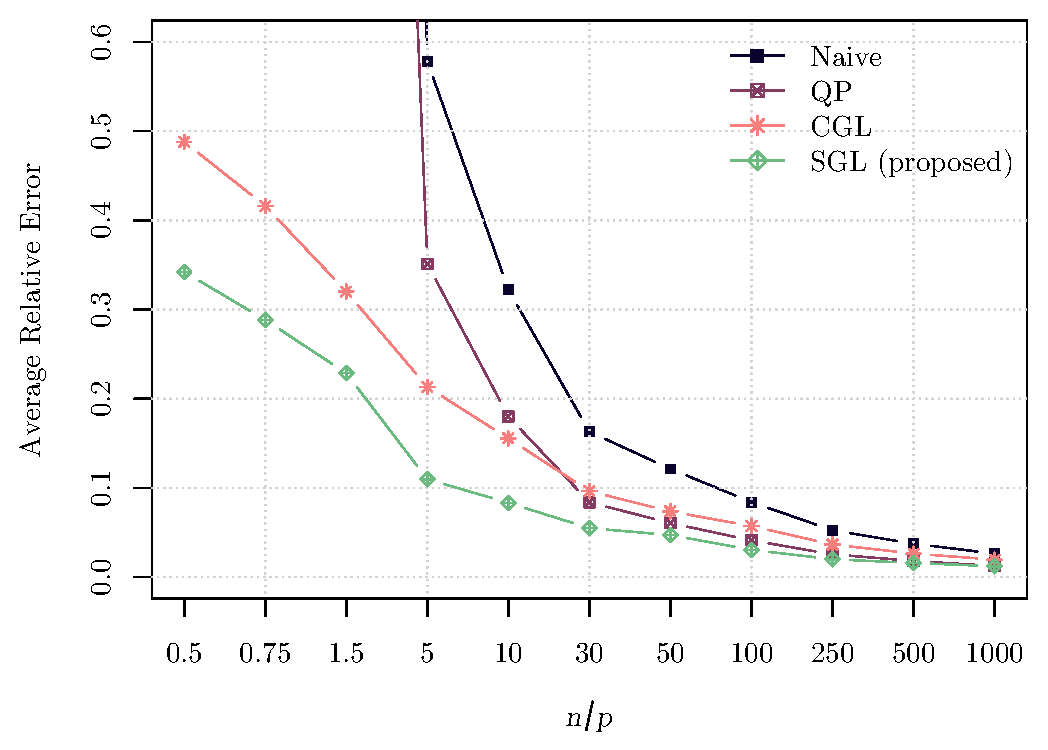
\includegraphics[width=\textwidth]{grid/latex/figures/relative_error_grid.eps}
    \end{subfigure}
    ~ %add desired spacing between images, e. g. ~, \quad, \qquad, \hfill etc.
      %(or a blank line to force the subfigure onto a new line)
    \begin{subfigure}[b]{0.47\textwidth}
        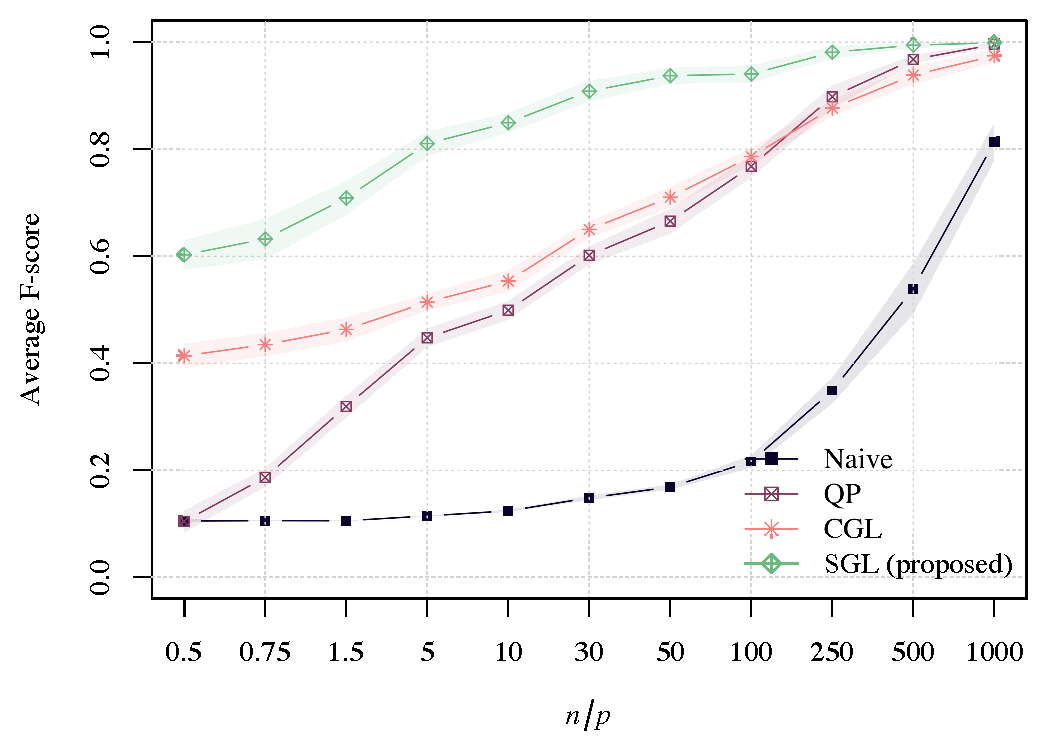
\includegraphics[width=\textwidth]{grid/latex/figures/fscore_grid.eps}
    \end{subfigure}
    \caption{Average performance results for learning Laplacian matrix of a $\mathcal{G}^{(64)}_{\mathsf{grid}}$.}
    \label{fig:performance-grid}
\end{figure}

Figure~\ref{fig:sample-grid} pictorially compares the graph structures learned by \textsf{SGL} and \textsf{CGL} when
$T/N = 100$.

\begin{figure}[!htb]
    \centering
    \begin{subfigure}[b]{0.3\textwidth}
        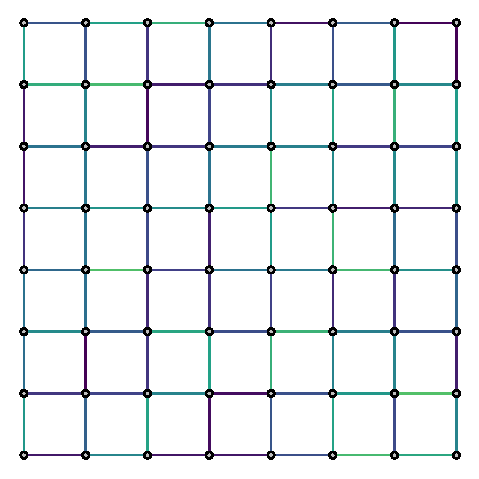
\includegraphics[width=\textwidth]{grid/latex/figures/true_grid.eps}
        \caption{Instance of a grid graph.}
    \end{subfigure}
    ~ %add desired spacing between images, e. g. ~, \quad, \qquad, \hfill etc.
      %(or a blank line to force the subfigure onto a new line)
    \begin{subfigure}[b]{0.3\textwidth}
        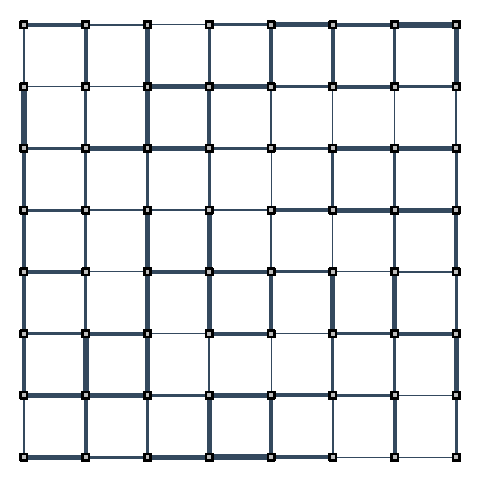
\includegraphics[width=\textwidth]{grid/latex/figures/sgl_grid.eps}
        \caption{\textsf{SGL} $(\mathsf{RE}, \mathsf{FS}) = (0.045, 0.982)$.}
    \end{subfigure}
    ~
    \begin{subfigure}[b]{0.3\textwidth}
        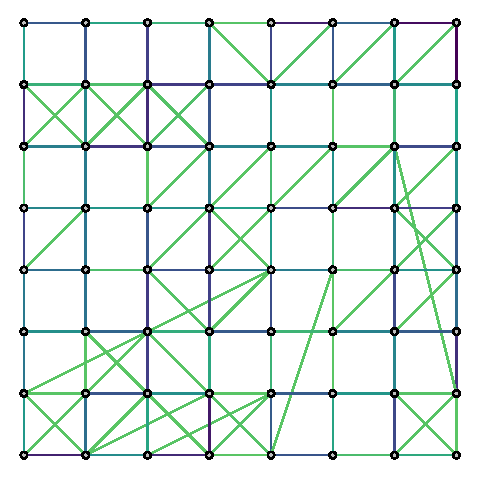
\includegraphics[width=\textwidth]{grid/latex/figures/cgl_grid.eps}
        \caption{\textsf{CGL} $(\mathsf{RE}, \mathsf{FS}) = (0.069, 0.812)$.}
    \end{subfigure}
    \caption{Sample results of learning $\mathcal{G}^{(64)}_{\mathsf{grid}}$ for $T/N = 100$. Edges smaller than $0.05$ were removed.
    For \textsf{SGL}, we fix $\beta = 10$, whereas for \textsf{CGL} we perform a grid search in $\alpha$ to find $\alpha$ that maximizes the F-score.
    We found $\alpha = 3.6\cdot 10^{-3}$.}
    \label{fig:sample-grid}
\end{figure}
